\documentclass[12pt]{article}
\usepackage{amsmath}
\usepackage{graphicx}
\usepackage{hyperref}
\usepackage[utf8]{inputenc}
\usepackage{geometry}
\usepackage{mathtools}
\usepackage{empheq}
\usepackage{listings}
\usepackage{xcolor}
\usepackage{minted}
\usepackage{svg}


\definecolor{LightGray}{gray}{0.9}

\graphicspath{ {./assets/} }
\geometry{margin=0.6in}

\title{CHEN 461 HW 1}
\author{Mark Levchenko}
\date{January 2023}

\begin{document}


\begin{enumerate}

% Problem 1 %%%%%%%%%%%%%%%%%%%%%%%%%%%%%%%%%%%%%%%%%%%%%%%%%%%%%%%%%%%%%%%%%%%%%%%%%%%
\newpage
\item Problem 3.2
\begin{enumerate}
    \item 
    \begin{align*}
        V \frac{dC_R}{dt} &= F C_{in,R} - F C_R - V k_R C_R^n \\
        C_R^n &\approx C_{R,s}^n + n C_{R,s}^{n-1} (C_R - C_{R,s}) \\
        \intertext{Deviation form:}
        \overline{C}_R^n &= n C_{R,s}^{n-1} \overline{C}_R \\
        V \frac{d\overline{C}_R}{dt} &= F \overline{C}_{in,R} - F \overline{C}_R - V k_R \overline{C}_R^n \\
        V \frac{d\overline{C}_R}{dt} &= F \overline{C}_{in,R} - F \overline{C}_R - V k_R n C_{R,s}^{n-1} \overline{C}_R \\
        V \frac{d\overline{C}_R}{dt} + \overline{C}_R \left( F  + V k_R n C_{R,s}^{n-1} \right) &= F \overline{C}_{in,R} \\
        \Aboxed{\frac{V}{F  + V k_R n C_{R,s}^{n-1}} \frac{d\overline{C}_R}{dt} + \overline{C}_R &= \frac{F}{F  + V k_R n C_{R,s}^{n-1}} \overline{C}_{in,R}}
    \end{align*}
    \item
    \begin{align*}
        \tau &= \frac{V}{F  + V k_R n C_{R,s}^{n-1}} \\
        k &= \frac{F}{F  + V k_R n C_{R,s}^{n-1}} \\
        \intertext{Transfer function:}
        \Aboxed{G(s) &= \frac{F}{Vs + F  + V k_R n C_{R,s}^{n-1}}}
    \end{align*}
    \item 
    \begin{align*}
        \intertext{Step input:}
        \overline{C}_{in,R}(t) &= M \mathcal{H}(t)
        \intertext{Step response:}
        y(t) &= kM (1 - e^{-t/\tau}) \\
        \Aboxed{\overline{C}_R(t) &= \frac{F M}{F  + V k_R n C_{R,s}^{n-1}} \left(1 - e^{-t/\left( \frac{V}{F  + V k_R n C_{R,s}^{n-1}} \right)}\right)}
    \end{align*}
\end{enumerate}

% Problem 2 %%%%%%%%%%%%%%%%%%%%%%%%%%%%%%%%%%%%%%%%%%%%%%%%%%%%%%%%%%%%%%%%%%%%%%%%%%%
\newpage
\item Problem 3.14
\begin{align*}
    A \frac{d\overline{h}}{dt} &= \overline{F}_{in} \\
    \overline{F}_{in} &= \frac{M}{\epsilon} (\mathcal{H}(t) - \mathcal{H}(t - \epsilon)) \\ 
    \mathcal{L}\left\{ A \frac{d\overline{h}}{dt} \right\} &= \mathcal{L}\left\{ \frac{M}{\epsilon} (\mathcal{H}(t) - \mathcal{H}(t - \epsilon)) \right\} \\
    As\overline{H}(s) &= \frac{M}{\epsilon} \left( \frac{1}{s} - \frac{e^{-\epsilon s}}{s} \right)\\
    \mathcal{L}^{-1}\left\{\overline{H}(s)\right\} &= \mathcal{L}\left\{\frac{M}{A \epsilon} \left( \frac{1}{s^2} - \frac{e^{-\epsilon s}}{s^2} \right)\right\} \\
    \Aboxed{\overline{h}(t) &= \frac{M}{A\epsilon} (t - (t - \epsilon) \mathcal{H}(t - \epsilon))}
\end{align*}

Here is a plot of what $\overline{h}(t)$ would look like:

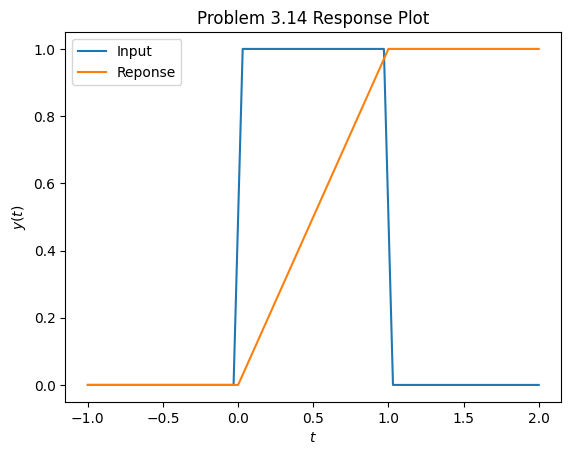
\includegraphics{461HW4_P314.png}

The response ramps up and reaches a new steady state. $\overline{h}(t)$ will not return to 0 as $t\rightarrow\infty$.

\newpage

Here is the code that generates the plot:

\begin{minted}[
framesep=2mm,
baselinestretch=1.2,
bgcolor=LightGray,
fontsize=\footnotesize,
breaklines,
]{python}
from sympy import lambdify, Heaviside
from sympy.abc import t

import numpy as np
import matplotlib.pyplot as plt

# convert sympy expressions to lambda func
u_expr = Heaviside(t) - Heaviside(t - 1)
u = lambdify(t, u_expr, 'numpy')

y_expr = t * Heaviside(t) - (t - 1) * Heaviside(t - 1)
y = lambdify(t, y_expr, 'numpy')

# plotting
t_ran = np.linspace(-1, 2, 100)

plt.plot(t_ran, u(t_ran))
plt.plot(t_ran, y(t_ran))
plt.xlabel(r"$t$")
plt.ylabel(r"$y(t)$")
plt.legend(['Input', 'Reponse'])
plt.title('Problem 3.14 Response Plot')
\end{minted}

% Problem 3 %%%%%%%%%%%%%%%%%%%%%%%%%%%%%%%%%%%%%%%%%%%%%%%%%%%%%%%%%%%%%%%%%%%%%%%%%%%
\newpage
\item Problem 3.17
\begin{enumerate}
    \item 
    \begin{align*}
        \mathcal{L}\left\{RC \frac{dV_C}{dt} + V_C\right\} &= \mathcal{L}\left\{V_{in}\right\} \\
        RCsV_C(s) + V_C(s) &= V_{in}(s) \\
        V_{out} &= V_{in} - V_C \\
        V_C &= V_{in} - V_{out} \\
         RCsV_{in}(s) - RCsV_{out}(s) + V_{in}(s) - V_{out}(s) &= V_{in}(s) \\
         V_{out}(s) (RCs + 1) &= RCsV_{in}(s) \\ 
         V_{out}(s) &= \frac{RCs}{RCs + 1} V_{in}(s) \\
         \Aboxed{G(s) &= \frac{RCs}{RCs + 1}} \\
    \end{align*}
    \item
    \begin{align*}
        \intertext{Response to step input:}
        V_C(t) &= kM\left(1 - e^{-t/\tau}\right) \\
        \tau &= RC \\
        k &= 1 \\
        V_C(t) &= M\left(1 - e^{-t/(RC)}\right) \\
        V_{in}(t) &= M\mathcal{H}(t) \\
        V_{out}(t) &= V_{in}(t) - M\left(1 - e^{-t/(RC)}\right) \\
        \Aboxed{V_{out}(t) &= M\mathcal{H}(t) - M\left(1 - e^{-t/(RC)}\right)}
    \end{align*}
    \item
    \begin{align*}
        V_{in}(t) &= M\sin(\omega t) \\
        \intertext{For large $t$:}
        V_C(t) &= \frac{kM}{\sqrt{1+(\omega \tau)^2}} \sin\left(\omega t - \tan^{-1}(\omega\tau)\right) \\
        \tau &= RC \\
        k &= 1 \\
        V_C(t) &= \frac{M}{\sqrt{1+(\omega RC)^2}} \sin\left(\omega t - \tan^{-1}(\omega RC)\right) \\
        V_{out}(t) &= V_{in}(t) - \frac{M}{\sqrt{1+(\omega RC)^2}} \sin\left(\omega t - \tan^{-1}(\omega RC)\right) \\
        \Aboxed{V_{out}(t) &= M\sin(\omega t) - \frac{M}{\sqrt{1+(\omega RC)^2}} \sin\left(\omega t - \tan^{-1}(\omega RC)\right)} \\
        \intertext{Account for phase shift:}
        \mathrm{Amplitude} &= \frac{M}{\sqrt{1+(\omega RC)^2}} \cdot \omega RC \\
        \mathrm{AR} &= \frac{\frac{M}{\sqrt{1+(\omega RC)^2}} \cdot \omega RC}{M} \\
        \Aboxed{\mathrm{AR} &= \frac{\omega RC}{\sqrt{1+(\omega RC)^2}}}
    \end{align*}

    Plot of AR v $RC\omega$:

    \includesvg{461HW4_P317.svg}

    The curve is flat at high frequency, "passing" those frequencies, and ramping the lower frequency up. The plot shows why the filter is called high pass.  
\end{enumerate}


% Problem 4 %%%%%%%%%%%%%%%%%%%%%%%%%%%%%%%%%%%%%%%%%%%%%%%%%%%%%%%%%%%%%%%%%%%%%%%%%%%
\newpage
\item
\begin{enumerate}
    \item 
    \begin{align*}
        \intertext{Implement algorithm:}
        \sigma_f[j] &= (1 - f) \sigma_f[j - 1] + f \sigma[j] \\ 
        f &= 1 - e^{\frac{-T_s}{\tau_f}}
    \end{align*}

    Here is a plot of the data with different $\tau_f$ values:

    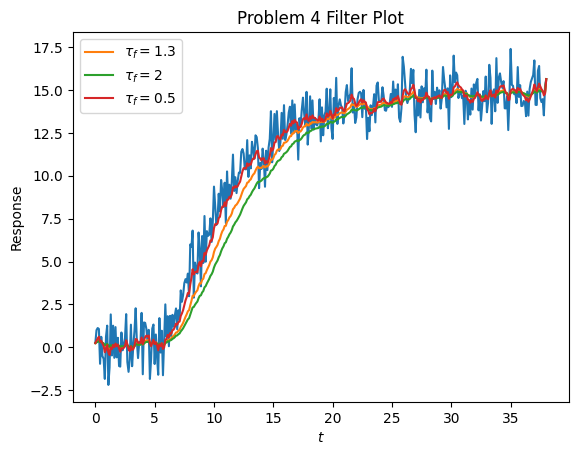
\includegraphics{461HW4_P4_1.png}

    At $\tau_f=0.5$ the data is not filtered enough; there is still significant variation. At $\tau_f=1.3$, the data is much smoother. At $\tau_f=2$, the data is even smoother, but the filtered data diverges significantly. $\tau_f=1.3$ is a good value if accuracy is desired. $\tau_f=2$ would be better if more smoothing of the data is desired.

\newpage

The code below implements the algorithm and produces the plot.

\begin{minted}[
framesep=2mm,
baselinestretch=1.2,
bgcolor=LightGray,
fontsize=\footnotesize,
breaklines,
]{python}
import numpy as np
from scipy.io import loadmat
import matplotlib.pyplot as plt
import math

# load data
data_file = loadmat('datafile.mat')

# low pass filter function
def lpf(t, y, tau_f):
    filt_y = y.copy()

    T_s = t[1] - t[0]
    f = 1 - math.exp(-T_s[0]/tau_f)

    # filter algorithm
    for i in range(1, len(y)-1):
        filt_y[i] = (1 - f) * filt_y[i-1,0] + f * y[i,0]

    return filt_y

# filter with different tau_f values
filt_1 = lpf(data_file['t'], data_file['y_data'], 1.3)
filt_2 = lpf(data_file['t'], data_file['y_data'], 2)
filt_3 = lpf(data_file['t'], data_file['y_data'], 0.5)

# plotting
plt.plot(data_file['t'], data_file['y_data'])
plt.plot(data_file['t'], filt_1, label=r"$\tau_f=1.3$")
plt.plot(data_file['t'], filt_2, label=r"$\tau_f=2$")
plt.plot(data_file['t'], filt_3, label=r"$\tau_f=0.5$")
plt.xlabel(r'$t$')
plt.ylabel('Response')
plt.legend()
plt.title('Problem 4 Filter Plot')
\end{minted}

    \item

    For a step input, one $\tau$ is the time at which the response reaches approximately 63.2\% of its maximum value. Looking at the data, the steady-state maximum is approximately 15. 63.2\% of 15 is 9.48. The response is 9.48 at approximately 11.5 min. The input started at 6 min, and so $\tau = 11.5 - 6$ = 5.5 min.


    The equation below is the response for a step input assuming a perfectly calibrated sensor.
    \[
        y(t) = M \cdot \left(1 -  e^{-t/\tau}\right)
    \]

    Test this equation against the data with $M=15$ and $\tau=5.5$.

    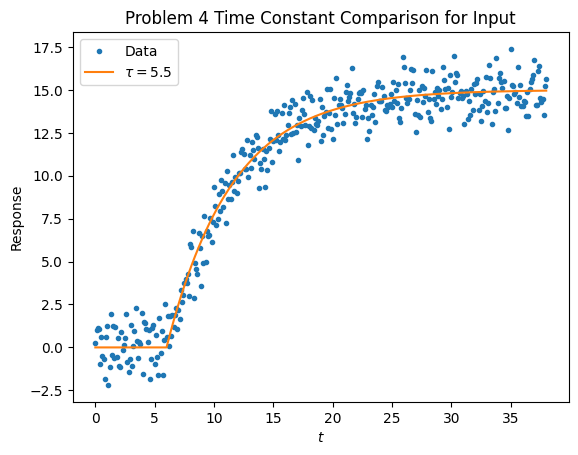
\includegraphics{461HW4_P4_2.png}

    The response output with $\tau=5.5$ fits the data reasonably well.

    $\boxed{\tau=5.5}$ is a suitable value.


    The code below creates the output for the plot.
    
\newpage

\begin{minted}[
framesep=2mm,
baselinestretch=1.2,
bgcolor=LightGray,
fontsize=\footnotesize,
breaklines,
]{python}
import numpy as np
from scipy.io import loadmat
import matplotlib.pyplot as plt
import math

# load data
data_file = loadmat('datafile.mat')

from sympy import Heaviside, exp, lambdify
from sympy.abc import t

# plot data
plt.plot(data_file['t'], data_file['y_data'], '.')

# create a response formula with tau=5.5
resp_expr = (15 * (1 - exp(-(t - 6) / 5.5))) * Heaviside(t - 6)
# convert expression to lamdba func
resp = lambdify(t, resp_expr, 'numpy')

# plotting
plt.plot(data_file['t'], resp(data_file['t']))
plt.title('Problem 4 Time Constant Comparison for Input')
plt.legend(['Data', r"$\tau=5.5$"])
plt.xlabel(r"$t$")
plt.ylabel("Response")
\end{minted}

\end{enumerate}




\end{enumerate}
\end{document}